\begin{figure}
\centering
\begin{subfigure}{0.45\textwidth}
\centering
\pgfmathsetmacro{\dm}{1/sqrt(5)}
\pgfmathsetmacro{\a}{1}
\pgfmathsetmacro{\b}{1}
\pgfmathsetmacro{\c}{1.5}
\pgfmathsetmacro{\aa}{sqrt(1-1/4)*\b}
\begin{tikzpicture}[font=\small,x={(-2*\dm cm,-\dm cm)},y={(2*\dm cm,-\dm cm)},z={(0,1cm)},declare function={f(\x)=\b*sqrt(1-1/(\a^2)*\x*\x);fa(\x)=\b*sqrt(1-1/(\a^2)*\x*\x-1/4);g(\x)=\c*sqrt(1-1/(\b^2)*\x*\x);h(\x)=\c*sqrt(1-1/(\a^2)*\x*\x);}]
\draw[-latex](0,0,0)--(\a+0.6,0,0)node[left]{$x$};
\draw[-latex](0,0,0)--(0,\b+0.6,0)node[right]{$y$};
\draw[-latex](0,0,0)--(0,0,\c+0.6)node[above]{$z$};
\draw[domain=-\a:\a]plot ({\x},{f(\x)},{0}) plot ({\x},{-f(\x)},{0});
\draw[domain=-\aa:\aa]plot ({\x},{fa(\x)},{\c/2}) plot ({\x},{-fa(\x)},{\c/2});
\draw[domain=-\b:\b]plot (0,\x,{g(\x)}) plot (0,\x,{-g(\x)});
\draw[domain=-\a:\a]plot (\x,0,{h(\x)}) plot (\x,0,{-h(\x)});
\draw(-0.4,{f(-0.4)},0)--++(0,0.5,0.5)node[right,align=center]{\RL{\عددی{xy} مستوی میں ترخیم}\\ $\frac{x^2}{a^2}+\frac{y^2}{b^2}=1$};
\draw(0,0.8,{-g(0.8)})--++(0,0.5,-0.25)node[right,align=center]{\RL{\عددی{yz} مستوی میں ترخیم}\\ $\frac{y^2}{b^2}+\frac{z^2}{c^2}=1$};
\draw({-0.7},{fa(-0.7)},{\c/2})--++(0,0.5,0.5)node[right,yshift=2ex,align=center]{\RL{مستوی \عددی{z=z_0} میں}\\   \RL{ترخیمی عمودی تراش}};
\draw(0,0,{0.5*\c})node[circ]{}node[left]{$z_0$};
\draw(\a,0,0)node[left,xshift=-0.5ex]{$a$};
\draw(0,\b,0)node[below,xshift=1ex]{$b$};
\draw(0,0,\c)node[above left]{$c$};
\end{tikzpicture}
\end{subfigure}\hfill
\begin{subfigure}{0.45\textwidth}
\centering
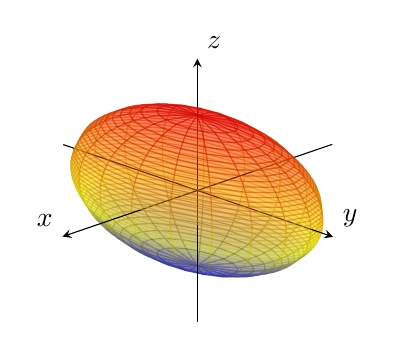
\begin{tikzpicture}
\pgfmathsetmacro{\a}{1}
\pgfmathsetmacro{\b}{1}
\pgfmathsetmacro{\c}{1.5}
\begin{axis}
[view={135}{20},%colormap/blackwhite,
axis lines=center, axis on top,ticks=none,
set layers=default,axis equal,
xlabel={$x$}, ylabel={$y$}, zlabel={$z$},
xlabel style={anchor=south east},
ylabel style={anchor=south west},
zlabel style={anchor=south west},
enlargelimits,
tick align=inside,
domain=0:2.00,
samples=20, 
z buffer=sort,
]
\addplot3 [surf,opacity=0.4,domain=-1:0,
domain y=0:360] ({sin(y)*sqrt(1-x^2)},{2*cos(y)*sqrt(1-x^2)},{x});
\addplot3 [surf,opacity=0.4,domain=0:1,domain y=0:360,on layer=axis foreground] ({sin(y)*sqrt(1-x^2)},{2*cos(y)*sqrt(1-x^2)},{x});
\end{axis}
\end{tikzpicture}
\end{subfigure}
\end{figure}


\begin{figure}
\centering
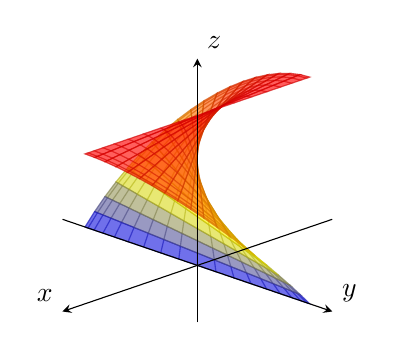
\begin{tikzpicture}
\pgfmathsetmacro{\a}{1}
\pgfmathsetmacro{\b}{1}
\pgfmathsetmacro{\c}{1}
\begin{axis}
[view={135}{20},%colormap/blackwhite,
axis lines=center, axis on top,ticks=none,
set layers=default,axis equal,
xlabel={$x$}, ylabel={$y$}, zlabel={$z$},
xlabel style={anchor=south east},
ylabel style={anchor=south west},
zlabel style={anchor=south west},
enlargelimits,
tick align=inside,
domain=0:2.00,
samples=20, 
z buffer=sort,
]
\addplot3 [surf,opacity=0.4,domain=0:360,
domain y=0:90] ({\a*sin(\x)*cos(\y)},{\b*sin(\x)*sin(\y)},{\c*cos(\y)});
%\addplot3 [surf,opacity=0.4,domain=0:1,domain y=0:360,on layer=axis foreground] ({sin(y)*sqrt(1-x^2)},{2*cos(y)*sqrt(1-x^2)},{x});
\end{axis}
\end{tikzpicture}
\end{figure}
